\documentclass[../../../analisi-dei-requisiti.tex]{subfiles}

\begin{document}

\subsubsection{AUC12: Aggiunta gestore}%
\label{subs:AUC12}

\begin{figure}[H]
  \centering
  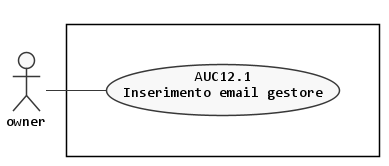
\includegraphics[width=100mm]{aggiunta-gestore.png}
  \caption{AUC12: Aggiunta gestore}%
  \label{fig:AUC12}
\end{figure}

\begin{description}
  \item[Codice:] AUC12;
  \item[Titolo:] Aggiunta gestore;
  \item[Attori primari:] owner;
  \item[Precondizione:] il sistema deve rendere disponibile la pagina per l'aggiunta del gestore, l'utente deve avere i requisiti per diventare gestore:
  \begin{enumerate}
    \item l'utente deve essere collegato o essersi collegato all'organizzazione nella quale svolgere il ruolo di gestore;
    \item l'utente deve essere un utente senza privilegi o un visualizzatore.
  \end{enumerate}
  \item[Postcondizione:] viene aggiunto il gestore specificato dall'owner;
  \item[Scenario principale:]
  \begin{enumerate}
    \item l'owner vuole aggiungere un gestore ad una delle sue organizzazioni.
  \end{enumerate}
\end{description}

\subsubsection{AUC12.1: Inserimento email gestore}%
\label{subs:AUC12.1}
\begin{description}
  \item[Codice:] AUC12.1;
  \item[Titolo:] Inserimento email gestore;
  \item[Attori primari:] owner;
  \item[Precondizione:] il sistema deve rendere disponibile la possibilità di inserire l'email del nuovo gestore;
  \item[Postcondizione:] l'email viene opportunamente inserita;
  \item[Scenario principale:]
  \begin{enumerate}
    \item l'owner inserisce l'email del nuovo gestore.
  \end{enumerate}
\end{description}

\end{document}
